\documentclass[12pt]{article}

\usepackage[margin=1in]{geometry}

\usepackage{mathtools,amsthm}
\DeclarePairedDelimiter\ceil{\lceil}{\rceil}
\DeclarePairedDelimiter\floor{\lfloor}{\rfloor}

\usepackage{fontspec}
\newfontfamily\cmunicode{CMU Serif}
\usepackage{microtype}

\usepackage[noend]{algpseudocode}
\usepackage{algorithm}
\newcommand*\Let[2]{\State #1 $\gets$ #2}
\newcommand*{\TO}{\textbf{to}}
% since gemm3 can't be a matro name
\newcommand*{\pluseq}{\mathrel{{+}{=}}}
\newcommand*{\gemmt}{{\textsc{gemm3}}}
\newcommand*{\gemmtp}{{\textsc{gemm3()}}}
\newcommand*{\gemm}{{\textsc{gemm}}}
\newcommand*{\gemmp}{{\textsc{gemm()}}}

\newcommand*{\mycite}[1]{~\cite{#1}}

\usepackage{hyperref}
\usepackage[maxbibnames=15]{biblatex}

\addbibresource{cites.bib}

\usepackage{setspace}
%\singlespacing{}
\doublespacing{}

\usepackage{graphicx}

\usepackage{tikz}
\usetikzlibrary{arrows.meta,calc,fit,positioning,chains}
\definecolor{l3-color}{cmyk}{0,0.06,0.12,0}
\definecolor{l2-color}{cmyk}{0,0.2,0.4,0}
\definecolor{l1-color}{cmyk}{0,0.45,0.55,0}
\definecolor{reg-color}{cmyk}{0.15,0.8,0.8,0}

\tikzset{bpack/.style={to path={
      foreach \i in {1,...,#1} { -- ++(0.5, 0) -- ++ (-0.5,-0.4) } -- (\tikztotarget) \tikztonodes
    }},
  bpack/.default=6,
  apack/.style={to path={
      foreach \i in {1,...,#1} { -- ++(0, -0.5) -- ++(0.4,0.5) } -- (\tikztotarget) \tikztonodes
    }},
  apack/.default=6}

\tikzset{
  label-brace/.style={to path={
      (\tikztostart) ++(#1) -- ++(#1)
      -- ($(\tikztotarget) + 2 *(#1)$) \tikztonodes
      -- +($-1 *(#1)$)
    }},
  brace below/.style={label-brace={0, -3pt}},
  brace above/.style={label-brace={0, 3pt}},
  brace right/.style={label-brace={3pt, 0}},
  brace left/.style={label-brace={-3pt, 0}}}

\tikzset{
  dim-label/.style={label distance=0pt,inner sep=0},
}

\tikzset{
  our-arrow/.style={-{Latex[length=8pt,width=4pt]}},
}

\tikzset{
  memory/.style={fill=white},
  l3/.style={fill=l3-color},
  l2/.style={fill=l2-color},
  l1/.style={fill=l1-color},
  regs/.style={fill=reg-color},
  legend/.style={on chain=labels, minimum height=1ex, minimum width=1em,
    draw, rectangle, outer sep=0, label={[label distance=3pt]right:{\small #1}}}
}

\tikzset{
  loop-label/.style={midway, draw, rectangle},
  square-mat/.style={rectangle,draw,fit={(0, 0) (3, -3)},inner sep=0},
  wide-mat/.style={rectangle,draw,fit={(0, 0) (3, -1)},inner sep=0},
  tall-mat/.style={rectangle,draw,fit={(0, 0) (1, -3)},inner sep=0}
}

\newcommand*{\bpackarr}[2][6]{\draw[our-arrow] ($(#2 - 0.75, -0.25)$) to[bpack=#1] ++($(0.5, -0.4 * #1)$);}
\newcommand*{\apackarr}[2][6]{\draw[our-arrow] ($(0.25, - #2 + 0.75)$) to[apack=#1] ++($(0.4 * #1, -0.5)$);}

\newcommand*{\bracelabel}[4]{\draw (#1) to[brace #3]%
  node[midway,label={[dim-label]#3:#4}] {} (#2);}

\newcommand*{\packlabel}[3]{\path (#1) -- (#2)%
  node[midway,label={#3:pack}] {};}

% [style] name width height N code-for-every
\newcommand*{\vgrids}[6][fill=white]{
  \foreach \x in {1, ..., #5} {
    \node[rectangle, draw, #1,fit={($(#3 * \x - #3, 0)$) ($(#3 * \x, -#4)$)}, inner sep=0] (#2\x) {};
    #6
  }
}
% [style] name width height N code-for-every
\newcommand*{\hgrids}[6][fill=white]{
  \foreach \y in {1, ..., #5} {
    \node[rectangle, draw, #1,fit={($(0, -\y * #4 + #4)$) ($(#3, -\y * #4)$)}, inner sep=0] (#2\y) {};
    #6
  }
}

% [first-style] style name width height N code-for-every
\newcommand*{\vgridscache}[7][memory]{
  \foreach \x in {1, ..., #6} {
    \ifnum\x=1%
    \node[rectangle, draw, #1 ,fit={($(#4 * \x - #4, 0)$) ($(#4 * \x, -#5)$)}, inner sep=0] (#3\x) {};
    \else
    \node[rectangle, draw, #2 ,fit={($(#4 * \x - #4, 0)$) ($(#4 * \x, -#5)$)}, inner sep=0] (#3\x) {};
    \fi
    #7
  }
}
% [first-style] style name width height N code-for-every
\newcommand*{\hgridscache}[7][memory]{
  \foreach \y in {1, ..., #6} {
    \ifnum\y=1%
    \node[rectangle, draw, #1,fit={($(0, -\y * #5 + #5)$) ($(#4, -\y * #5)$)}, inner sep=0] (#3\y) {};
    \else
    \node[rectangle, draw, #2,fit={($(0, -\y * #5 + #5)$) ($(#4, -\y * #5)$)}, inner sep=0] (#3\y) {};
    \fi
    #7
  }
}

\newcommand*{\pluseqnode}[1]{\node[at={(0, -1.5)}] (#1-plus) {\large $\pluseq$};}

% [style] N N - 1 offset-right
\newcommand*{\loopborder}[3][black]{\draw[rounded corners, color=#1]%
  (#2-loop.west) -| ($(#3-rect-west) + (-5pt, -5pt)$) coordinate (#2-rect-west)%
  -- ($(#3-rect-east) + (5pt, -5pt)$) coordinate (#2-rect-east)%
  |- (#2-loop.east);}


\title{\gemmt{}: Constant-Workspace High-Performance Multiplication of Three Matrices for Matrix Chaining\\
{\large Honors Thesis in Partial Fulfillment of the Turing Scholars Degree Program}}
\author{Krzysztof A. Drewniak}

\begin{document}
\maketitle{}
\begin{abstract}
  The generalized matrix chain problem considers how to efficiently compute a series of matrix multiplications where some of the operands may be inverted, transposed, or have mathematical properties that can be used to increase performance.
  Solutions to this problem often involve series of calls to high-performance implementations of matrix multiplication (\gemm{}).
  We introduce a primitive, \gemmt{}, which multiplies three general matrices, to aid in solving this problem.
  By taking advantage of the structure of modern algorithms for \gemm{}, we derive an algorithm for \gemmt{} which can multiply three matrices using only a constant amount of additional memory.
  Current approaches to such multiplications require a temporary buffer than can be arbitrarily large.
  We present experimental results which show that our algorithm retains performance comparable to that of current methods.
\end{abstract}

\section{Introduction}
The matrix chain problem asks how to efficiently parenthesize a matrix product $A_1A_2\cdots A_N$.
$O(N \log N)$ algorithms for solving this problem are known\mycite{Hu1984}, as are simpler $O(N^3)$ dynamic-programming solutions\mycite{Barthels2018}.
These algorithms all assume that the only operation available is the multiplication of two matrices.

In practice, a more general version of this problem appears, where matrices can be transposed and/or inverted, or have properties such as being upper triangular\mycite{Barthels2018}.
For example, an algorithm to compute the ensemble Kalman filter\mycite{Rao2017} (which computes parameters for physical systems from noisy data) requires the computation of the expression $X_i^b S_i (Y_i^b)^T R_i^{-1}$, which features one transposition and one inverse.
Other examples of the generalized matrix chain problem include the expression $L^{-1}AL^{-H}$ (where $L$ is lower triangular and $A$ is symmetric), which is known as the two-sided triangular solve\mycite{Poulson2011} and $\tau_u\tau_v vv^TAuu^T$ (where the $\tau_i$ are scalars and $v$ and $u$ are vectors), which appears in an algorithm for reducing a matrix to tridiagonal form\mycite{Choi1995}.

The BLAS\mycite{blas_standard} and LAPACK\mycite{lapack_ug} libraries provide many high-performance functions that can assist in the computation of such matrix chains, such as specialized functions for the multiplication of triangular matrices (\textsc{trmm}).
However, manually determining how to use these functions and coding in term of them requires expert knowledge.
Existing high-level systems, such as Matlab and Julia, which are commonly used by non-experts, generally compute generalized matrix chains in a naive way, such as proceeding from left to right, which is often ineffecient.
Systems such as Linnea\mycite{Barthels2017} have emerged recently that attack the generalized matrix chain problem and automatically generate a high-performance program for a given expression in term of high-performance operations such as matrix-matrix multiply.

Returning to the example matrix chains above, we can observe that they often contain the multiplication of three matrices as a subproblem, often after some preprocessing such as an inversion or an outer product.
The general form of such a problem is $G \coloneqq \alpha DEF + \beta G$ (with some of the operands optionally transposed), which we will summarize as $G \pluseq DEF$ and denote \gemmt{}, by analogy with the notation for general matrix-matrix multiply (\gemm{}) in the BLAS library.
The letters $D$, $E$, $F$, and $G$ were chosen to avoid confusion with discussions of \gemm{}, which has the form $C \pluseq AB$.
The only approach available for this subproblem with current methods is to parenthesize the expression $DEF$ and perform a pair of matrix multiplications, storing a result in a temporary matrix $T$.
This method has two drawbacks.
The first is that $T$ is often rather large (and could be larger than some or all the input matrices) and thus requires significant amounts of storage space.
In addition, if $T$ is sufficiently large, creating and using it incurs a non-negligible overhead due to the large number of slow main-memory operations required.

To combat these issues, we have developed an algorithm for \gemmt{} which does not require an entire intermediate product to be computed and stored at one time.
Our algorithm takes advantage of the blocking performed by modern \gemm{} implementations to only store a cache-sized block of $EF$ at any given time.
By doing so, we perform the multiplication in $O(1)$ additional space and maintain performance comparable with a pair of \gemm{} calls.
Our algorithm can therefore be used as a primitive in generalized matrix chain solvers (or hand-written matrix code) to reduce memory usage, decrease the complexity of the solution, and potentially provide a slight performance increase.

\section{Background}
\subsection{High-performance {\cmunicode \gemm{}}}
Before discussing our approach to \gemmt{}, it is important to review the implementation of high-performance \gemm{}.
High-performance \gemm{} algorithms operate by repeatedly reducing the multiplication to a series of multiplications of regions of the inputs.
These regions are sized to allow an operand to one of these subproblems to utilize a level of the CPU's cache effectively and prevent it from being evicted during further subdivision.
Multiple levels of such subdivision are required to effectively utilize all levels of the cache.
These steps are necessary because of the memory hierarchy of modern CPUs, where there are multiple (currently three) levels of cache, which increase in size but decrease in speed, between registers and main memory.
Subdividing the matrices in a matrix multiplication along some dimension and then computing each resulting subproblem is known as \emph{partitioning} along that dimension.

The process of subdividing the operands to \gemm{} is intended to produce regions with particular shapes that can be computed with high performance or will lead to such shapes.
If we consider a $m' \times n'$ subregion $M'$ of a matrix $M$, we will say that $M'$ is a \emph{block} of $M$ if $m'$ and $n'$ are approximately equal.
If $m'$ is much smaller than $n'$, then $M'$ is a \emph{row panel}, while having $n'$ much smaller than $m'$ makes $M'$ a \emph{column panel} of $M$.

There are two specialized primitives that appear in high-performance \gemm{}: the \emph{microkernel} and \emph{macrokernel}.
The microkernel is a highly-tuned, hand-written function (almost always implemented in assembly) that multiplies an $m_R \times k$ row panel of $A$ by a $k \times n_R$ column panel of $B$ to update an $m_R \times n_R$ block of $C$, which is updated in registers and written to memory.
An illustration of the microkernel is located in Algorithm \ref{alg:macrokernel}.
(In this illustration, as with all others in this work, constants that appear twice indicate the dimension along which each loop proceeds, along with the stride.)
The parameters $m_R$ and $n_R$ are based on the microarchitecture of the CPU, which can be derived analytically\mycite{Low2016} or by autotuning\mycite{Whaley1998}.

\begin{algorithm}
  \caption{The macrokernel of a high-performance \gemm{} implementation.}
  \label{alg:macrokernel}
  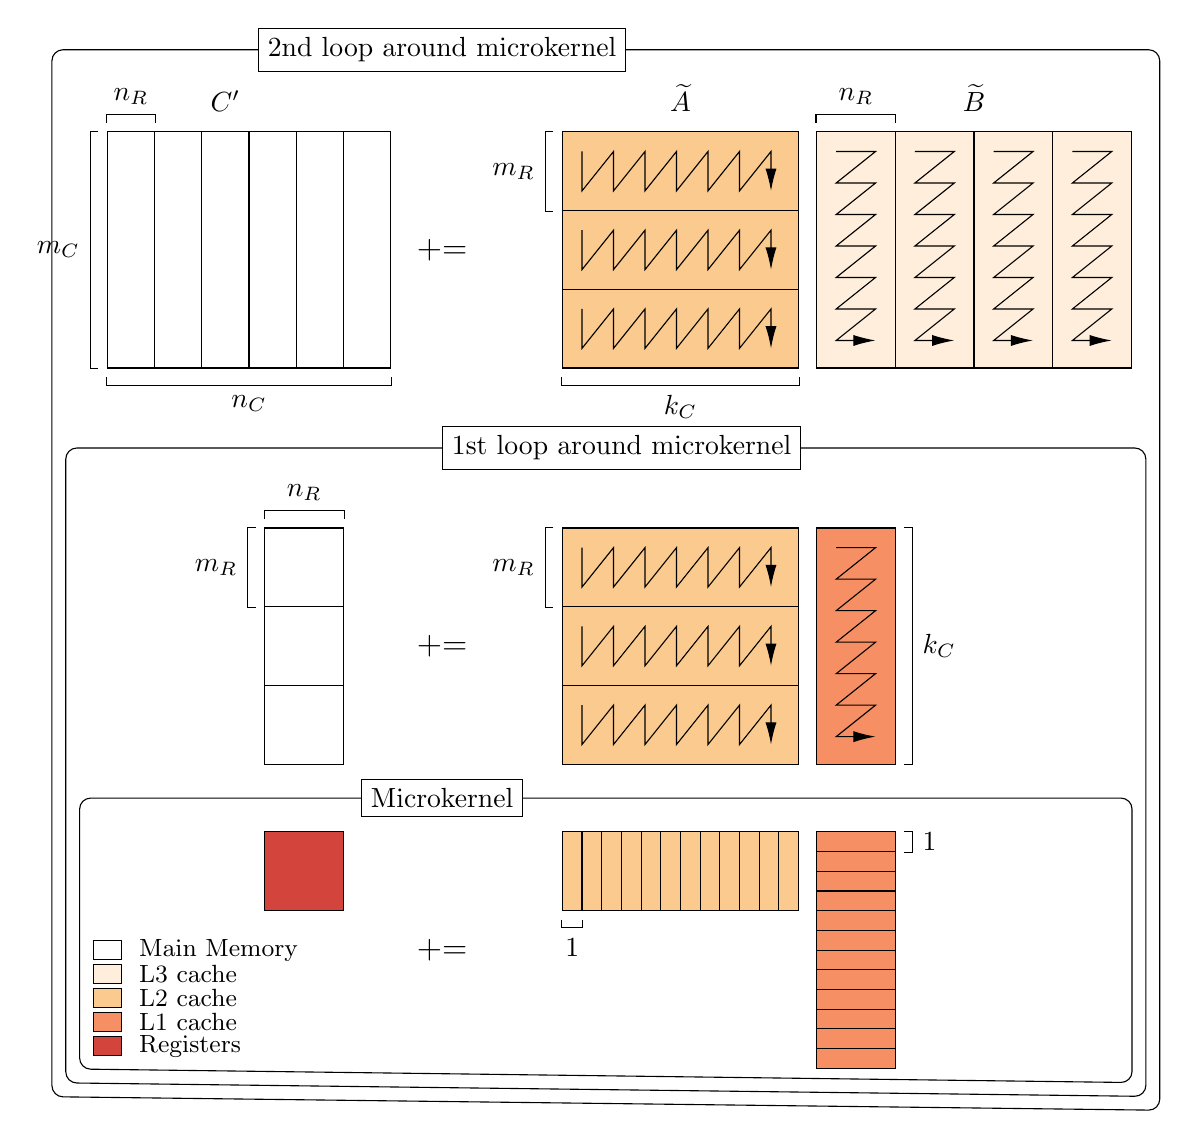
\begin{tikzpicture}
    \matrix (loops)[column sep=0.2cm, row sep=5.5ex] {
  \vgrids[memory]{2C}{0.6}{3}{6}{}
  \bracelabel{2C1.north west}{2C1.north east}{above}{$n_R$}
  \bracelabel{2C1.south west}{2C6.south east}{below}{$n_C$}
  \bracelabel{2C1.north west}{2C1.south west}{left}{$m_C$}
  \path (2C1.north west) -- (2C5.north east) node[midway,label={above:$C'$}] {};&

  \pluseqnode{2}&

  \hgrids[l2]{2A}{3}{1}{3}{\apackarr{\y}}
  \bracelabel{2A1.north west}{2A1.south west}{left}{$m_R$}
  \bracelabel{2A3.south west}{2A3.south east}{below}{$k_C$}
  \path (2A1.north west) -- (2A1.north east) node[midway,label={above:$\widetilde{A}$}] {};&

  \vgrids[l3]{2B}{1}{3}{4}{\bpackarr{\x}}
  \bracelabel{2B1.north west}{2B1.north east}{above}{$n_R$}
  \path (2B1.north west) -- (2B4.north east) node[midway, label={above:$\widetilde{B}$}] {};\\

  \foreach \y in {1,...,3} {
    \node[rectangle, draw, fit={(2, -\y + 1) (3, -\y)}, inner sep=0] (1C\y) {};
  }
  \bracelabel{1C1.north west}{1C1.south west}{left}{$m_R$}
  \bracelabel{1C1.north west}{1C1.north east}{above}{$n_R$}&

  \pluseqnode{1}&

  \hgrids[l2]{1A}{3}{1}{3}{\apackarr{\y}}
  \bracelabel{1A1.north west}{1A1.south west}{left}{$m_R$}&

  \vgrids[l1]{1B}{1}{3}{1}{\bpackarr{\x}}
  \bracelabel{1B1.north east}{1B1.south east}{right}{$k_C$}\\


  \node[rectangle, draw, regs, fit={(2, 0) (3, -1)}, inner sep=0] (0C) {};
  \begin{scoped}[start chain=labels going {below=2pt of \tikzchainprevious}]
    \node[legend=Main Memory, memory] at (0, -1.5) {};
    \node[legend=L3 cache, l3] {};
    \node[legend=L2 cache, l2] {};
    \node[legend=L1 cache, l1] {};
    \node[legend=Registers, regs] {};
  \end{scoped}&

  \pluseqnode{0}&

  \vgrids[l2]{0A}{0.25}{1}{12}{}
  \bracelabel{0A1.south west}{0A1.south east}{below}{$1$}&

  \hgrids[l1]{0B}{1}{0.25}{12}{}
  \bracelabel{0B1.north east}{0B1.south east}{right}{$1$}\\
};
\path node[draw,above=2cm of 2-plus] (2-loop) {2nd loop around microkernel}
(2-plus) -- (1-plus) node[loop-label,anchor=west] (1-loop) {1st loop around microkernel}
(1-plus) -- (0-plus) node[loop-label] (0-loop) {Microkernel};

\draw[rounded corners] let \p1 = ($(0B12.south east) + (0pt, -5pt)$),
\p2 = ($(2B4.south east) + (0pt, -5pt)$),
\p{east} = (\x2, \y1) in
(0-loop.west) -| ($(labels-end.south west) + (-5pt, -5pt)$) coordinate (0-rect-west)
-- (\p{east}) coordinate (0-rect-east)
|- (0-loop.east);

\loopborder{1}{0}
\loopborder{2}{1}

  \end{tikzpicture}
  \begin{algorithmic}
    \Procedure{macrokernel}{$\widetilde{A}, \widetilde{B}, C'$}
    \For{$j \gets 0, n_R, \ldots$ \TO{} $n_C$}
    \For{$i \gets 0, m_R, \ldots$ \TO{} $m_C$}
    \State{using the microkernel}
    \State{$C'[i:i + m_R, j:j + n_R] \pluseq \widetilde{A}[i:i+m_R,:] \cdot \widetilde{B}[:,j:j+n_R]$}
    \EndFor{}
    \EndFor{}
    \EndProcedure{}
  \end{algorithmic}
\end{algorithm}

Before being passed to the microkernel, the values in the input matrices must undergo \emph{packing}, that is, rearrangement into the specialized packed storage order also illustrated in Algorithm \ref{alg:macrokernel}.
One reason for this is that, to ensure efficiency, the data in each panel on which the microkernel operates must be arranged so that it is read in a linear fashion, which is the pattern of reads best suited to the CPU's memory prefetcher.
This is achieved by storing each panel of $A$ in column-major form with columns of height $m_R$ and keeping each panel of $B$ row-major with row width $n_R$.
Since this is not the typical storage format of a matrix, we must rearrange a series of panels from the input into this packed format before calling the microkernel.

A larger contributor to the efficiency of the microkernel is that the packed panels it operates on were resident in cache before the microkernel was called.
Since caches are fixed-size, we can only store a fixed number of these panels at any given time.
Specifically, we can only store an $m_C \times k_C$ subregion of $A$ and a $k_C \times n_C$ subregion of $B$.

We will use $\widetilde{A}$ and $\widetilde{B}$ to denote the packed regions of $A$ and $B$, respectively, and $C'$ to denote the corresponding block of $C$.
The loops that perform $C' \pluseq \widetilde{A}\widetilde{B}$ form the macrokernel, which is depicted as Algorithm \ref{alg:macrokernel}.
(In all the algorithms presented in this work, we will use Python-style notation for indexing, that is, matrices are 0-indexed and   $M[a:b, c:d]$ selects rows $[a, b)$ and columns $[c, d)$, with omitted operands spanning to the beginning/end of the dimension.)

The parameters $m_C$, $k_C$, and $n_C$ are chosen to ensure all levels of cache are used efficiently.
The process of choosing these parameters, described in Section \ref{subsec:params}, leaves $m_C$ close in size to $k_C$ and keeps $n_C$ much larger then both of these.
This means that $\widetilde{A}$ corresponds to a block of $A$, while $\widetilde{B}$ is a rearranged row panel of $B$.

Many high-performance \gemm{} implementations in use today are based on Goto's algorithm\mycite{Goto2008}.
One such implementation, which we have based our work on, is BLIS\mycite{VanZee2016}.
The BLIS algorithm, which is a refactoring of Goto's algorithm, is presented as Algorithms \ref{alg:macrokernel} and  \ref{alg:blis}.
It brings the row panel of $B$ into the $L3$ cache (later moving its constituent column panels into $L1$), while storing a block of $A$ in $L2$.
\begin{algorithm}
  \caption{The BLIS algorithm}
  \label{alg:blis}
  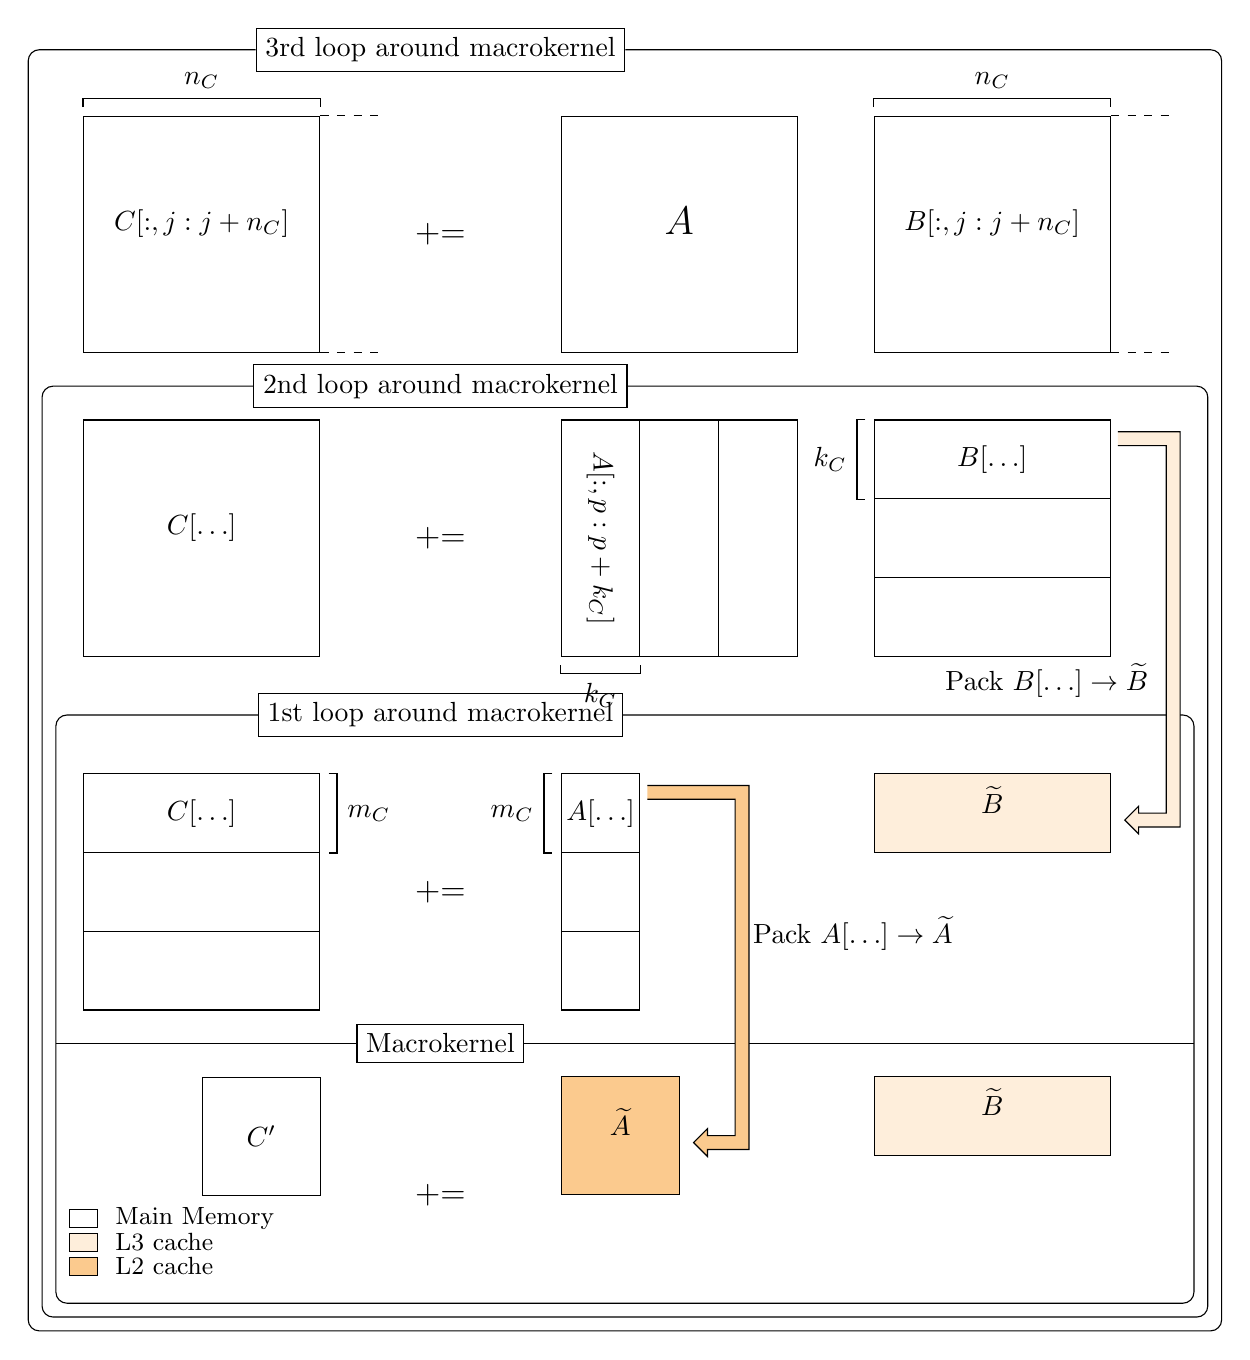
\begin{tikzpicture}
    \matrix (loops)[column sep=0.2cm, row sep=5.5ex] {
  \node[square-mat] (3C) {$C[:,j:j+n_C]$};
  \bracelabel{3C.north west}{3C.north east}{above}{$n_C$}
  \draw[dashed] (3C.north east) -- ++(0.75, 0)
  (3C.south east) -- ++(0.75, 0);&

  \pluseqnode{3}&

  \node[square-mat,memory] (3A) {\Large $A$};&

  \node[square-mat,memory] (3B) {$B[:,j:j+n_C]$};
  \bracelabel{3B.north west}{3B.north east}{above}{$n_C$}
  \draw[dashed] (3B.north east) -- ++(0.75, 0)
  (3B.south east) -- ++(0.75, 0);\\


  \node[square-mat,memory] (2C) {$C[\ldots]$};&

  \pluseqnode{2}&

  \vgrids[memory]{2A}{1}{3}{3}{}
  \node[at=(2A1),rotate=-90] {$A[:,p:p+k_C]$};
  \bracelabel{2A1.south west}{2A1.south east}{below}{$k_C$}&

  \hgrids[memory]{2B}{3}{1}{3}{}
  \node[at=(2B1)] {$B[\ldots]$};
  \bracelabel{2B1.north west}{2B1.south west}{left}{$k_C$}\\


  \hgrids[memory]{1C}{3}{1}{3}{}
  \node[at=(1C1)] {$C[\ldots]$};
  \bracelabel{1C1.north east}{1C1.south east}{right}{$m_C$}&

  \pluseqnode{1}&

  \hgrids[memory]{1A}{1}{1}{3}{}
  \node[at=(1A1)] {$A[\ldots]$};
  \bracelabel{1A1.north west}{1A1.south west}{left}{$m_C$}&

  \node[l3,wide-mat] (1B) {$\widetilde{B}$};\\

  \node[rectangle,draw,memory,at={(1.5, 0)},anchor=north west,minimum height=1.5cm, minimum width=1.5cm] (0C) {$C'$};
  \begin{scoped}[start chain=labels going {below=2pt of \tikzchainprevious}]
    \node[legend=Main Memory, memory] at (0, -1.8) {};
    \node[legend=L3 cache, l3] {};
    \node[legend=L2 cache, l2] (legend-anchor) {};
  \end{scoped}&

  \pluseqnode{0}&

  \node[l2,tall-mat,fit={(0, 0) (1.5, -1.5)}] (0A) {$\widetilde{A}$};&

  \node[l3,wide-mat,  wide-mat/.style={rectangle,draw,fit={(0, 0) (3, -1.5)},inner sep=0},] (0B) {$\widetilde{B}$};\\
};
\path node[draw,above=1.8cm of 3-plus] (3-loop){3rd loop around macrokernel}
(3-plus) -- (2-plus) node[loop-label] (2-loop){2nd loop around macrokernel}
(2-plus) -- (1-plus) node[loop-label] (1-loop) {1st loop around macrokernel}
(1-plus) -- (0-plus) node[loop-label] (0-loop) {Macrokernel};

\draw[rounded corners] let \p1 = ($(labels-end.south) + (0pt, -10pt)$),
\p2 = ($(0B.south east) + (30pt, 0)$),
\p3 = ($(labels-end.south west) + (-5pt, 0)$),
\p{east} = (\x2, \y1), \p{west} = (\x3, \y1) in
(1-loop.west) -| (\p{west}) coordinate (1-rect-west)
-- (\p{east}) coordinate (1-rect-east)
|- (1-loop.east);

\loopborder{2}{1}
\loopborder{3}{2}

\draw let \p1 = (0-loop),
\p2 = (1-rect-west),
\p3 = (1-rect-east),
\p{west-end} = (\x2, \y1),
\p{east-end} = (\x3, \y1) in
(0-loop.east) -- (\p{east-end})
(0-loop.west) -- (\p{west-end});

\path[draw, l3] (2B1.east) ++(2.5pt, 5pt) coordinate (B-arr-start)
-| ($(1B.east) + (20pt, 0pt)$) node[pos=0.82,left=3pt] {Pack $B[\ldots] \to \widetilde{B}$} coordinate (B-arr-down)
-- ++ (-10pt, 0)
-- ++(0pt, 2.5pt) -- ++(-5pt, -5pt) -- ++(5pt, -5pt) -- ++(0, 2.5pt)
-- ($(B-arr-down) + (5pt, -5pt)$)
|- ($(B-arr-start) + (0pt, 5pt)$);

\path[draw, l2] (1A1.east) ++(2.5pt, 5pt) coordinate (A-arr-start)
-| ($(0A.east) + (20pt, 0pt)$) node[pos=0.7,right=3pt] {Pack $A[\ldots] \to \widetilde{A}$} coordinate (A-arr-down)
-- ++ (-10pt, 0)
-- ++(0pt, 2.5pt) -- ++(-5pt, -5pt) -- ++(5pt, -5pt) -- ++(0, 2.5pt)
-- ($(A-arr-down) + (5pt, -5pt)$)
|- ($(A-arr-start) + (0pt, 5pt)$);

  \end{tikzpicture}
  \begin{algorithmic}
    \Procedure{BLIS\_gemm}{$A, B, C$}
    \For{$j \gets 0, n_C, \ldots$ \TO{} $n$}
    \For{$p \gets 0, k_C, \ldots$ \TO{} $k$}
    \State{pack $B[p:p+k_C,j:j+n_C] \to\widetilde{B}$}
    \For{$i \gets 0, m_C, \ldots$ \TO{} $m$}
    \State{pack $A[m:m+m_C,p:p+k_C] \to \widetilde{A}$}
    \State{$\textsc{macrokernel}(\widetilde{A}, \widetilde{B}, C[i:i+m_C,j:j+n_C])$}
    \EndFor{}
    \EndFor{}
    \EndFor{}
    \EndProcedure{}
  \end{algorithmic}
\end{algorithm}

\subsection{Parameter selection for the BLIS algorithm}\label{subsec:params}
The parameters $m_R$, $n_R$, $k_C$, $m_C$, and $n_C$ that appear in the BLIS algorithm are computed using an analytical model from \mycite{Low2016}.
We will summarize the process of deriving some of these parameters here.
The values of $m_R$ and $n_R$ determine the structure of the microkernel, and are derived from the width of vector registers on a given CPU along with the latency and throughput of fused-multiply-add (FMA) instructions.
Since we are reusing existing optimized microkernels, we will not detail the process of selecting these parameters in this work.

The process of selecting the remaining parameters assumes that, for each cache level $i$, the $L_i$ cache has is a $W_{Li}$-way set-associative cache with $N_{Li}$ sets and $C_{Li}$ bytes per cache line.
All the caches are also assumed to have a least-recently-used replacement policy.
$S_{elem}$ represents the size of a single element of the matrix for generality.

The first parameter we can derive is $k_C$, as it appears deepest in the loop structure of the algorithm.
We know that we will load a different $n_R \times k_C$ panel of $\widetilde{B}$ from $L1$ during each call to the microkernel.
We also know that the microkernel's reads from an $m_R \times k_C$ panel of $\widetilde{A}$ will cause it to be resident in the $L1$ cache.
Finally, some values from $C'$ will also enter the cache, and must not evict the panels.

To prevent the panels of $\widetilde{A}$ and $\widetilde{B}$ from evicting each other from the $L1$ cache, we want them to reside in different ways within each cache set.
To achieve this, the panels of $\widetilde{A}$ and $\widetilde{B}$ must both have sizes that are integer multiples of $N_{L1}C_{L1}$.
This restriction, along with the size of the data in each panel, tells us that
\begin{equation*}
  m_Rk_CS_{elem} = C_AN_{L1}C_{L1}
\end{equation*}
for some integer $C_A$, and that the same relationship holds for $n_R$ and $B$.

Given the three sources of data in the $L1$ cache, it must be the case that $C_A + C_B + 1 \leq W_{L1}$ (the $1$ is for elements of $C'$), and that we want to maximize $C_B$ given this constraint.
Therefore, we have
\begin{equation*}
  C_B = \ceil*{\frac{n_Rk_CS_{elem}}{N_{L1}C_{L1}}} = \ceil*{\frac{n_R}{m_R}C_A}.
\end{equation*}
Manipulating the inequality further shows us that
\begin{equation*}
  C_A \leq \floor*{\frac{W_{L1} - 1}{1 + \frac{n_R}{m_R}}}.
\end{equation*}

Choosing the largest possible value of $C_A$ that leaves $k_C$ an integer will maximize $k_C$, improving performance by increasing the amount of time spent in the microkernel.
Here we note that the process of deriving $m_R$ and $n_R$ leaves us the freedom to swap $m_R$ and $n_R$ (thus inverting the $n_R/m_R$ term above) if it would improve the value of $C_A$ without incurring a performance penalty.

Now that we have $k_C$, we can compute $m_C$ and $n_C$.
For $m_C$, we know that we need to reserve one way in the $L2$ cache for elements of $C'$, and $\ceil*{(n_Rk_CS_{elem})/(N_{L2}C_{L2})} = C_{B2}$ ways for the panel of $B$ in the $L1$ cache.
This allows us to bound $m_C$ by
\begin{equation*}
  m_C \leq \floor*{\frac{(W_{L2} - C_{B2} - 1)N_{L2}C_{L2}}{k_CS_{elem}}}
\end{equation*}
and then select $m_C$ as large as possible, keeping in mind that it must be divisible by $m_R$ for high performance.

Since the $L3$ cache is, in practice, very large and somewhat slow, $n_C$ is computed by finding the largest value such that $n_Ck_C$ is less that the size of the $L3$ cache, excluding an $L1$ cache's worth of space to allow elements of $C'$ or $\widetilde{A}$ to pass through.

\subsection{Data reuse in  matrix multiplication}
Examining the loops in the BLIS algorithm, as was done in\mycite{Low2016}, shows that each loop causes some data from the computation to be reused, that is, read or written in its entirety during each iteration of the loop.
For example, the microkernel reuses the small block of $C'$ that is stored in registers while looping over the panels.

Even though reuse occurs at each level of the algorithm, we will focus on the reuse of the packed buffers, as this is a key consideration for maintaining the performance of the algorithm, as shown by \mycite{Henry92}.
Packing into $\widetilde{B}$ and $\widetilde{A}$ introduces overhead, which is time that is not usable for computation.
Therefore, reusing the packed buffers many times will lower the relative proportion of time spent on packing, thus increasing performance.

Consider the multiplication $C \pluseq AB$, where $A$ is $m \times k$ and $B$ is $k \times n$.
To improve reuse of $\widetilde{B}$ during this computation, we need the first loop around the macrokernel, which packs into $\widetilde{A}$, to run many times, since each of those iterations covers computations that read the entirety of $\widetilde{B}$.
That is, we need $m$ to be large, as small values of $m$ will hurt performance by reducing the time between successive $\widetilde{B}$ packing operations.
Similarly, large values of $n$ allow the second loop around the microkernel to execute many times, thus improving reuse of $\widetilde{A}$, which is consumed by the first loop around the microkernel.

The only loops that iterate over $k$ are those that pack $\widetilde{B}$ (the second loop around the macrokernel) and the microkernel.
The second loop around the macrokernel does not result in the reuse of any data that has been loaded into cache because it is the first loop that performs such loads.
The microkernel only reuses data in registers, and so does not reuse cached data.
However, if $k$ is much less than $k_C$, the microkernel will only iterate a few times, increasing the proportion of time spent on non-computational overhaed.
Therefore, the size of $k$ has little impact on the reuse of packed blocks, except when $k \ll k_C$.

This reasoning shows that the BLIS algorithm achieves its best performance when $m$ and $n$ are large and $k$ near a multiple of $k_C$.

\section{Algorithm}
For our discussion of \gemmt{}, we well be considering the operation $G \pluseq DEF$, where $D$ is $m \times k$, $E$ is $k \times l$ and $F$ is $l \times n$.

\subsection{Deriving {\cmunicode \gemmt{}}}
To derive our algorithm for \gemmt{}, we considered $\gemm{}(D, EF, G)$, with the BLIS algorithm, looking for when elements of $EF$ were needed and whether it was possible to only compute parts of that product as necessary.
We define the computation of $G \pluseq D(EF)$ to be the \emph{outer algorithm}, and the operations needed to compute parts of $E \cdot F$ when needed to be the \emph{inner algorithm}.
Analyzing the outer algorithm showed that the earliest we would need to read from $EF$ was the step where \gemm{} packs $B$ to $\widetilde{B}$, and so the inner algorithm would need to compute the appropriate part of $B = EF$ before this step.

The first step of the \gemm{} algorithm reduces $C \pluseq AB$ (or, in our case, $G \pluseq D(EF)$) to the following subproblems:
\begin{equation*}
  \left[\begin{array}{c|c|c|c|c|c}
    C_{,1}&C_{,2}&\cdots&C_{,j}&\cdots& C_{n \mod n_C}
  \end{array}\right]
  = A
  \left[\begin{array}{c|c|c|c|c|c}
    B_{,1}&B_{,2}&\cdots&B_{,j}&\cdots&B_{n \mod n_C}
  \end{array}\right].
\end{equation*}
If we substitute in the values we are computing with, we have:
\begin{equation*}
  \left[\begin{array}{c|c|c|c|c|c}
    G_{,1}&G_{,2}&\cdots&G_{,j}&\cdots& G_{n \mod n_C}
  \end{array}\right]
  = D\left(
    E
    \left[\begin{array}{c|c|c|c|c|c}
      F_{,1}&F_{,2}&\cdots&F_{,j}&\cdots&F_{n \mod n_C}
    \end{array}\right]
  \right).
\end{equation*}

Now, for the $j$th subploblem, the matrices will be partitioned in the $k$ dimension as follows:
\begin{equation*}
  C_{,j}
  =
  \left[\begin{array}{c|c|c|c|c|c}
    A_{,1}&A_{,2}&\cdots&A_{,p}&\cdots&A_{,k \mod k_C}
  \end{array}\right]
  \left[\begin{array}{c}
    B_{1,j}\\\hline
    \vdots\\\hline
    B_{p,j}\\\hline
    \vdots\\\hline
    B_{k \mod k_C,j}
  \end{array}\right].
\end{equation*}
For the \gemmt{} computation, we have
\begin{equation*}
  G_{,j}
  =
  \left[\begin{array}{c|c|c|c|c|c}
    D_{,1}&D_{,2}&\cdots&D_{,p}&\cdots&D_{,k \mod k_C}
  \end{array}\right]
  \left(
  \left[\begin{array}{c}
          E_{1,}\\\hline
          \vdots\\\hline
          E_{p,}\\\hline
          \vdots\\\hline
          E_{k \mod k_C,}
  \end{array}\right]
  F_{,j}
  \right).
\end{equation*}

At this point in the algorithm, the subregion $B_{p, j}$ is a row panel of $B$ with a fixed size that will be packed into $\widetilde{B}$, which resides in $L3$ cache.
We cannot, however, pack from $(EF)_{p, j}$, as we have not computed these values.
However, if we examine the regions of $E$ and $F$ that correspond to $B_{p, j}$, we notice that $E_{p,}$ is a $k_C \times l$ row panel of $E$ and that $F_{,j}$ is an $l \times n_C$ block of $F$ (under typical conditions), which is a multiplication that can be performed efficiently.

Since the next step in the BLIS algorithm requires the region $(EF)_{p, j}$ to be computed, we must either compute this region now or compute $EF_{,j}$ during the previous loop.
Computing during the previous loop would result in an arbitrarily large product, preventing us from attaining the memory savings we were searching for.
However, the product $E_{p,}F_{,j}$ comprises $k_Cn_C$ floats, which can be stored in $O(1)$ memory.
This shows that the current point in the \gemm{} algorithm is the only time in which we can compute a subregion of $EF$ while keeping the algorithmic properties we sought.

\subsection{The inner algorithm}
Now that we have identified the computations that the inner algorithm must perform, we must turn to the problem of deriving it.

The multiplication of a row panel by a block is one that can be carried by the BLIS algorithm without a significant performance loss despite a somewhat suboptimal shape.
Therefore, an initial approach to computing $(EF)_{p, j} = E_{p,}F_{,j}$ would be to reuse the BLIS algorithm, nesting it within the outer computation.
However, in order to ensure performance, we need to make several changes to the BLIS algorithm.
The simplest change is to remove the redundant outermost loop of the inner algorithm, since $n$ cannot be more than $n_C$ for its inputs.

The next change we must make is to instruct the microkernel to write its output in the packed format by informing it the output matrix is stored in row-major form with width $n_R$.
This allows us to avoid having to pack the output of the inner algorithm, eliminating a large number of otherwise required memory operations and the corresponding overhead.
The change allows us to write $\widetilde{EF}$ directly, eliminating the ``pack $\widetilde{B}$'' step from the outer algorithm.
Therefore, we can simply consider the inner algorithm to be performing the operation $\widetilde{EF} = E_{p,}F_{,j}$.

We must also use an $n_C$ value equal to half of the $n_C$ value derived for the BLIS algorithm for both the inner and outer algorithms.
This prevents the packed panels of $\widetilde{F}$ from evicting the output $\widetilde{EF}$ from $L3$ cache, where it needs to reside in order to satisfy the assumptions of the outer algorithm.
The inner algorithm must place its output in $L3$ cache to prevent unnecessary memory operations from being performed.
This change to $n_C$ does not  break the assumptions of the BLIS algorithm, as $n_C/2$ is still much larger than $k_C$ or $m_C$ in practice.

The other parameter adjustment that needs to be performed is to reduce $k_C$ so that it is divisible by $m_R$ if that is not already the case.
If this is not done, the BLIS macrokernel's loops will have a final iteration that considers fewer than $m_R$ rows during each invocation of the inner algorithm since $k_C$ becomes the $m$ dimension for the inner problem.
Computation of this fringe iteration has a performance impact, as special processing is required to account for the unusual sizes, especially since the loop that this cost would normally be amortized over only runs for a few iterations in the inner algorithm.
This gains from eliminating this source of low performance outweigh the losses from having a slightly suboptimal $k_C$ value.
However, $l_C$, which is the inner algorithm's version of $k_C$, can be kept at the BLIS value, as these performance considerations do not arise in this stark fashion there.

It should be noted that one flaw in our approach is that the inner computation is a panel-matrix multiply, that is, the $m$ dimension is small, and $\widetilde{F}$ sees little reuse.
This suboptimal shape did have a performance impact, though it turned out to be small in practice.

The algorithm that results from this derivation is Algorithm \ref{alg:gemm3}, which is illustrated in Figure \ref{fig:gemm3}.

\begin{figure}
  \centering
  \includegraphics[height=8.5in]{gemm3-picture}
  \caption{Illustration of algorithm for \gemmt{}. Constants that appear twice indicate the dimension along which each loop proceeds, along with the stride.}
  \label{fig:gemm3}
\end{figure}
\begin{algorithm}
  \caption{Algorithm for \gemmt{}}
  \label{alg:gemm3}
  \begin{algorithmic}
    \Procedure{gemm3}{$D, E, F, G$}
    \For{$j \gets 0, n_C, \ldots$ \TO{} $n$}
    \For{$p \gets 0, k_C, \ldots$ \TO{} $k$}
    \For{$q \gets 0, l_C, \ldots$ \TO{} $l$}
    \State{pack $F[q:q+l_C,j:j+n_C] \to \widetilde{F}$}
    \For{$i \gets 0, m_C, \ldots$ \TO{} $k_C$}
    \State{pack $E[i:i+m_C,q:q+l_C] \to \widetilde{E}$}
    \State{$\textsc{macrokernel}(\widetilde{E}, \widetilde{F}, \widetilde{EF})$}
    \Comment{writes in packed form}
    \EndFor{}
    \EndFor{}
    \For{$i \gets 0, m_C, \ldots$ \TO{} $m$}
    \State{pack $D[m:m+m_C,p:p+k_C] \to \widetilde{D}$}
    \State{$\textsc{macrokernel}(\widetilde{D}, \widetilde{EF}, G[i:i+m_C,j:j+n_C])$}
    \EndFor{}
    \EndFor{}
    \EndFor{}
    \EndProcedure{}
  \end{algorithmic}
\end{algorithm}

\subsection{Variations for similar problems}
It is important to note that this algorithm computes $G \pluseq D(EF)$.
In some cases, it is much more efficient (on account of the dimensions of the inputs) to compute $G \pluseq (DE)F$ instead.
Attempting to derive an algorithm for that problem directly does not work, as the block $\widetilde{DE}$ in $L2$ is not of a shape that can be multiplied efficiently by the BLIS algorithm.
Fortunately, we can transform problems of this form to the equivalent problem $G^T \pluseq F^T(E^TD^T)$.
This transformation can be performed at effectively no cost by re-interpreting the memory the matrices are stored in (treating a matrix stored in row-major form as column-major and vice-versa).

\section{Experiments and Results}
\subsection{Implementation}
To test our algorithm's performance, we implemented both it and the BLIS algorithm in the Multilevel Optimization for Matrix Multiply Sandbox (MOMMS), which was developed for\mycite{SmithDiss2017}.
This framework allowed us to declaratively generate the code for an algorithm by specifying the series of loops and packing operations required, and allowed us to interface to the BLIS microkernels.
Initially, we verified that the MOMMS implementation of the BLIS algorithm had similar performance to the reference implementation, which was written in C.
Then, we modified the MOMMS framework to support generating code for multiplying three matrices.
These modifications allowed us to express both our \gemmt{} algorithm and the typical $T = EF; G \pluseq DT$ method we were comparing against.

We tested the performance, in billions of floating point operations (GFLOPS) per second, of both our algorithm and the typical approach.
The target machine had an Intel Xeon E3-1270 v3 CPU, which ran at 3.5 GHz and implemented the Haswell microarchitecture.
The experimental system had 15 GB of RAM, 8 MB of $L3$ cache, 256 KB of $L2$ cache (which was an 8-way set-associative cache with 64 byte cache lines) and 32 KB of $L1$ cache (per core, with the same associativity and line sizes as the $L2$ cache).
The theoretical peak performance of this system on matrix multiplication is 56 GFLOPS per second, which is the top of the y-axis on all out performance plots.
The blocking parameters that arose from this data can be found in Table \ref{tab:parameters}

\begin{table}
  \centering
  \begin{tabular}{l|c c}
    &\gemmt{}&BLIS algorithm\\ \hline
    $m_R$&6&6\\
    $n_R$&8&8\\
    $m_C$&72&72\\
    $k_C$&252&256\\
    $l_C$&256&\\
    $n_C$&2040&4080\\
  \end{tabular}
  \caption{Blocking parameters for the Haswell microarchitecture}
  \label{tab:parameters}
\end{table}

\subsection{Experiments performed}
Our experiments were run both on square matrices ($m = n = k = l = N$, where $D$ is $m \times k$, $E$ is $k \times l$, $F$ is $l \times n$, and $G$ is $m \times n$) and on problems where a particular dimension was fixed at $252$ while the others varied together, to evaluate the performance of these algorithms on multiple input shapes.
The parameter $252$ was chosen for the rectangular case because it was $k_C$ for the \gemmt{} algorithm and slightly below $l_C$ and the $k_C$ value for BLIS.
We sampled the performance at multiples of sixteen from $N = 16$ to $4912$ to test the suitability of our approach on many input sizes.
All the inputs were stored in column-major form, while the temporaries and outputs were stored in row-major form, since the BLIS microkernel has noticably increased performance when writing to row-major matrices (and since the packed buffer is row-major).
This unusual combination of input formats ensured a fair comparison between the two algorithms.
In addition, we tested the $G^T = F^T(E^TD^T)$ case, in which all matrices were row major, for square inputs.

A plot of the computed additional memory consumption (excluding inputs and outputs) for multiplying square matrices using both algorithm is shown in Figure \ref{fig:bc_square_mem}, demonstrating our approach's much lower memory usage.

The results of these experiments can be found in Figure \ref{fig:bc_square} for square matrices, and Figure \ref{fig:bc_rectangles} for the rectangular inputs.
The $G \pluseq (DE)F$ experiment's results are in Figure \ref{fig:ab_square}.
Data for the square case shows that, once performance has stabilized around $N = 512$, the two algorithms are almost always within 5\% of each other in GFlops/s, showing comparable performance.

\begin{figure}
  \centering
  \includegraphics[height=0.40\textheight]{../results/earwig2/gemm3_memory}
  \caption{Memory usage of our \gemmt{} implementation compared to a pair of \gemm{} calls}
  \label{fig:bc_square_mem}
\end{figure}

\begin{figure}
  \centering
  \includegraphics[height=0.40\textheight]{../results/earwig2/gemm3}
  \caption{Performance of our \gemmt{} implementation compared to a pair of \gemm{} calls, square matrices}
  \label{fig:bc_square}
\end{figure}

\begin{figure}
  \centering
  \includegraphics[width=0.95\textwidth]{../results/earwig-correct-rectangle-flops/gemm3_rectangles}
  \caption{Performance of our \gemmt{} implementation compared to a pair of \gemm{} calls, rectangular matrices}
  \label{fig:bc_rectangles}
\end{figure}

\begin{figure}
  \centering
  \includegraphics[height=0.40\textheight]{../results/earwig2/gemm3_ab_bc_kernel}
  \caption{Performance of our \gemmt{} implementation compared to a pair of \gemm{} calls, square transposed matrices}
  \label{fig:ab_square}
\end{figure}

\subsection{Analysis}
From the figures in the previous section, it is clear that \gemmt{} attains similar performance to a pair of \gemm{} calls with significantly lower memory usage.
However, it is important to dissect these performance results and determine why they have arisen.

For the square case, which was shown in Figure \ref{fig:bc_square}, we can observe that, for most of the 1000s and 2000s, the pair of \gemm{} calls has somewhat increased performance, but that the \gemmt{} algorithm has comparable or higher performance afterwards.
The higher performance for the \gemm{} calls arises from the lack of reuse of $\widetilde{F}$ implied by the $252 \times l \cdot l \times n$ input to the inner algorithm for \gemmt{}.
Specifically, the first loop around the macrokernel in that algorithm always iterates at most four times, compared to the unbounded number of iterations in a call to \gemm{} to compute $EF$.
However, around when the temporary grows to 64 MB, the memory cost of writing it to memory becomes large enough that the performance of two \gemm{} calls begins to drop to and eventually falls below the performance of our \gemmt{} algorithm.
This shows that our approach, in addition to the memory savings, provides performance benefits for large matrix multiplications.

For small input sizes ($N < 512$), there is often a significant performance benefit attained by the \gemmt{} algorithm.
This performance improvement arises from the additional packing step that a pair of \gemm{} calls must perform, which has a non-negligible cost for these inputs, even if both the packed and unpacked data remain resident in the $L3$ cache.

Similar trends can be seen in Figure \ref{fig:ab_square}, which shows the results for $G \pluseq (DE)F$, implemented as $G^T \pluseq F^T(E^TD^T)$.
However, the pair of \gemm{} calls retains higher performance for a longer period of time on this workload.
This occurs because packing from row-major matrices to row-major packed buffers, which is something that occurs more frequently in this experiment, is much more amenable to the CPU's prefetcher than packing from column-major matrices.

The rectangular-matrix results from Figure \ref{fig:bc_rectangles} also require examination.
When $k$ is at or around $k_C$, the \gemmt{} algorithm performs better on all inputs, as the low $\widetilde{F}$ reuse issues that normally impact the performance of our algorithm now also affect the performance of the \gemm{} calls while our performance advantages from lower memory usages remain.
When the $n$ dimension is narrow, the outer problem in the \gemmt{} algorithm eventually becomes a column-panel times block multiply, which creates an extremely slight performance drop (never more than 2\%) against the pair of matrix-column panel multiplies from the \gemm{} calls.

When the $m$ dimension is narrow, we see the effects of suboptimal parenthesization, as both algorithms must perform a matrix-matrix multiply followed by a vector-matrix multiply once the dimensions other than $n$ are large enough.
The performance of both algorithms is equal because both are primarily affected by the memory-bound nature of the computation.
Similarly, if $l$ is narrow, the computations are approximately outer product followed by a matrix-matrix multiply, which could be performed much more efficiently by moving the parentheses, as shown by the narrow $k$ case.

These results demonstrate the general suitability of our algorithm for \gemmt{} and its suitability as a high-performance primitive.

\section{Conclusions}
We have demonstrated that, by exploiting the structure of the BLIS algorithm for matrix-matrix multiplication, we can derive an algorithm for \gemmt{} (multiplying three matrices together) that only requires a constant amount of additional memory.
We have shown that, while the basic concept of our algorithm arises naturally from the structure of \gemm{}, several tweaks are needed to retain high performance.

Experimental results have indicated that, on a variety of workloads, our algorithm maintains a similar level of performance to existing approaches to this problem.
We know that, on sufficiently small or large problems of certain shapes, our approach offers increased performance because it eliminates a source of memory operation overhead.
However, there are input sizes that are known to have a small negative performance impact on our approach due to the suboptimal multiplication shape our approach used as a subproblem.
Neither these gains or losses are particularly large, so we conclude that the main advantages of our approach are the memory savings it offers.

An additional improvement offered by \gemmt{} is that it introduces a cleaner programming interface for the multiplication of three matrices, which is a problem that often arises in practice.
Therefore, our algorithm will give both programmers and authors of linear algebra code generators (such as Linnea\mycite{Barthels2017}) an interface that is easier to invoke and does not require the manual allocation of a temporary buffer.

\paragraph{Future Work} This work only investigates a sequential implementation of \gemmt{}.
In the future, we intend to investigate how we can efficiently parallelize our \gemmt{} algorithm to take advantage of the multiple CPU cores available on modern CPUs.
We also plan to verify the portability of our results by testing on multiple different CPU microarchitectures, such as the recent Knight's Landing processors from Intel.

\paragraph{Acknowledgments}
We would like to thank Prof.\ Robert van de Geijn for advising this research and directing us towards the research question.
We also wish to thank Dr.\ Tyler Smith for writing MOMMS and assisting with the algorithm design, and Prof.\ Tze Meng Low for his advice on resolving certain performance issues.
Finally, we wish to acknowledge National Science Foundation for funding this work through awards CCF-1714091, ACI-1550493, and CCF-1320112.
% \section{Things that still might need doing}
% \begin{itemize}
% \item Portability (run on KNL)
% \item Clean experiments (public lab machines are kinda a bad place)
% \item Parallel case (the square-case performance behavior we have is still there, just much more exaggerated on multiple cores)
% \item Make this somewhat longer to keep the writing flag people happy (should happen if we fix one of these other points)
% \end{itemize}
\printbibliography{}
\end{document}
